\documentclass[11pt]{article}
\usepackage{times}
\usepackage{graphicx}
\usepackage{enumerate}
\usepackage{amsmath}
\usepackage{amsthm}
\usepackage{amsbsy}
\usepackage{amsfonts}




\renewcommand{\labelenumii}{\arabic{enumii}.}

\evensidemargin=-.25in \oddsidemargin=-0.25in \topmargin=-1in
\textheight=9.0in \textwidth=7.0in
\parindent=0pt
\parskip=5pt

\begin{document}
	
	\begin{center}
		\rule{7.3in}{2pt}
		{\large AI 533 \hfill {\bf Intelligent Agents and Decision Making~~~~~} \hfill Winter 2025}\\[2pt]
		OREGON STATE UNIVERSITY\\
		School of Electrical Engineering and Computer Science \\ [2pt]
		Instructor: Sandhya Saisubramanian\\
		\rule{7.3in}{2pt}
	\end{center}
	
	\vskip 0.2in
	\begin{center}
	\large Total points: 100 \hfill	{\large Assignment 1: MDP  } \hfill \large Due date: Jan 27, 2025
	\end{center}
	
	\vskip 0.2in
	
	\thispagestyle{empty}
	
	\textbf{Instructions}: Collaboration is not allowed on any part of this assignment. It is acceptable to discuss concepts or clarify questions but you must document who you worked with for this assignment. Copying answers or reusing solutions from individuals/the internet is unacceptable and will be dealt with strictly. 
	Solutions must be typed (hand written and scanned submissions will not be accepted) and saved as a .pdf file. 
	
	\begin{enumerate}
	
	\item \textbf{(15 points)} MDP design.  For the following example scenarios, you must (1) write a factored state representation, discuss if it is discrete or continuous, and whether your state representation satisfies the Markov property; (2) \textit{list} the actions (e.g.  move up, move right, etc.) the agent should have to accomplish the assigned task;  (3) write a reward function such that optimizing the reward function will help the agent accomplish its task efficiently (optimally)  and briefly explain your answer. You are free to choose $R(s)$, $R(s,a)$ or $R(s,a,s')$ for your reward function. You can write your reward function mathematically or describe it clearly in text.  Proposed reward functions must be reasonable, practical, and must not lead to unsafe behavior. 
	
	(i) A robotic vacuum cleaner is assigned the task of removing dirt from the floor
	
	(ii) A legged robot wants to run a marathon and reach the finish line as quickly as possible
	
	(iii) An autonomous car whose decisions must minimize the mean commute for all drivers (those driven by humans and those driven by AI)
	
	(iv) An underwater robot that must monitor the health of corals
	
	(v) An autonomous robot that is tasked with irrigating and fertilizing the crops to maximize crop yield, without adversely affecting crop and soil health. 
	
	\item \textbf{(15 points)} Given an MDP $M = (S,A,T,R,\gamma)$ with a fixed state state $s_0$ and a fixed policy $\pi$, the probability that the action at time $t=0$ is $a\in A$ is:
	\[ \Pr(A_0 =a) = \pi(s_0, a). \] Similarly, the probability that the state at time $t=1$ is $s\in S$ is: \[ \Pr(S_1=s) = \sum_{a_0 \in A} \pi(s_0,a_0) T(s_0,a_0,s).\]
	
	Write a similar mathematical expression (using only $S,A,T,R,\gamma,\pi$ and Bayes' theorem ) for the following:
	
		(i) The  expected reward at time $t=6$ given that the action at time $t=3$ is $a\in A$ and the state at time $t=5$ is $s \in S$. Use $R(s,a)$ for reward notation.
		
		(ii) The probability that the action at time $t=16$ is $a' \in A$ given that the action at time $t=15$ is $a\in A$ and the state at time $t=14$ is $s \in S$. 

	
	\item  \textbf{(5 points)} How many deterministic policies (optimal or otherwise) exist for an MDP with 5 states and 10 actions?
	
	

	\item \textbf{(10 points)} For the MDP in the following figure with one state and one action, let $R(s_1) = 0$ and $V_0(s_1) = 5$. (i) Will value iteration converge when $\gamma=1$? Briefly explain your answer. (ii) Will value iteration converge when $\gamma=0.9$? Briefly explain your answer.
	
		\begin{figure}[h]
		\centering
		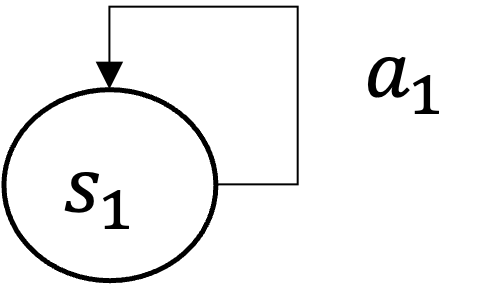
\includegraphics[scale=0.65]{mdp1.png}
	\end{figure}
	
	\item \textbf{(15 points)} Prove the following two statements mathematically or provide an example to demonstrate the property.  \\
  Statement 1: Multiplying all rewards (of a finite, discrete MDP with bounded rewards) by a positive scalar does not change the optimal policy. \\Statement 2: Adding a positive constant to all rewards (all states or state-action pairs or state-action-successor pairs in the MDP) of a finite MDP with bounded rewards changes the optimal policy. 
	
	\item  \textbf{(30 points)} In this question, the goal is to demonstrate that value improvement in value iteration is not monotonic. While the values and the policy converge to optimal at termination, for a finite, bounded MDP, the values (and the resulting policy) before convergence of value iteration are not guaranteed to improve in a monotonic manner. 
	
	Consider the MDP in Figure~\ref{fig:MDP} with four states, five actions that have deterministic transitions, and discount factor $\gamma=1$. The reward for being in each state, $R(s)$, is reported in the table in Figure~\ref{fig:MDP}.  Let $V_i$ and $V_{i+1}$ denote value functions from two  iterations of value iteration on this problem \textbf{before convergence}. Let  $\pi_i$ and $\pi_{i+1}$ denote the policies that are greedy with respect to these value functions. 
	
	
	(i) You are required to assign an initial value ($V_0$) to each of the state such that the expected reward following the greedy policy is not monotonic, $\pi_{i+1} < \pi_i$. Initialize $V_0$ such that at some finite iteration count $i$ before convergence of VI, the expected reward following $\pi_{i+1}$ is less than the expected reward following $\pi_i$, causing a change in the \textit{current} optimal action at least in one state.
	
	For example, let $a_1$ and $a_2$ denote the actions available in state $s$. Let the true optimal action in $s$ be $a^*=a_1$. You must initialize $V_0$ such that at iteration $i$, the policy that is greedy on the values $\pi(s) = a_1$ but at iteration $i+1$, $\pi(s) = a_2$ and in some $i+k$, the policy stabilizes to the true optimal policy $\pi(s) =a_1$.
	
	(ii) Show your calculation of value iteration to support (i). 
	
	
	\begin{figure}[h]
		\centering
		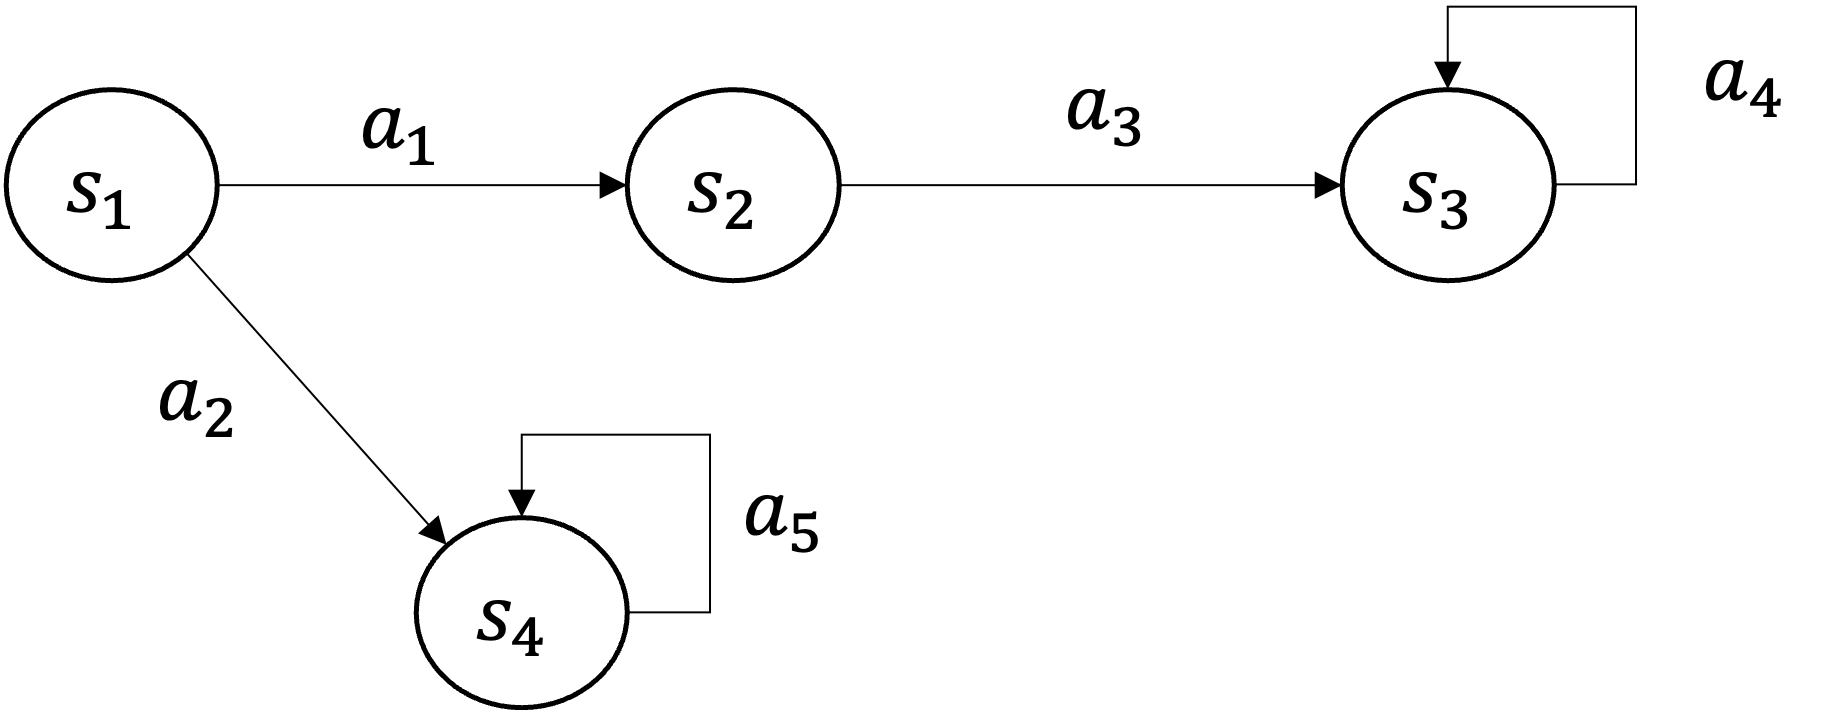
\includegraphics[scale=0.5]{mdp-1.png}
		
\includegraphics[scale=0.5]{mdp-1-reward.png}
		\caption{Graph for analyzing monotonicity of value iteration}
		\label{fig:MDP}
	\end{figure}
	
	
	\item \textbf{(10 points)} In class, we proved the contraction mapping for the Bellman equation, independent of the policy. You are required to prove that the Bellman backup operator for a particular policy converges. 
	For a deterministic policy $\pi$ and $0 \leq \gamma <1$ , let us define a contraction operator $(B^\pi V)(s) = R(s,\pi(s))+\gamma \sum_{s'} T(s,\pi(s),s') V(s')$. Prove that $\left \Vert B^\pi V - B^\pi V'\right \Vert \leq \gamma \left \Vert V- V'\right \Vert$. Hint: use the max-norm operator $\Vert v \Vert = max_s |v(s)|$ and follow steps similar to the proof in lecture slides. 
	\end{enumerate}
	
	
\end{document}